\documentclass[a4paper,12pt,twoside]{memoir}

% Castellano
\usepackage[spanish,es-tabla]{babel}
\selectlanguage{spanish}
\usepackage[utf8]{inputenc}
\usepackage[T1]{fontenc}
\usepackage{lmodern} % Scalable font
\usepackage{microtype}
\usepackage{placeins}
\usepackage[table,xcdraw]{xcolor}
\usepackage{adjustbox}
\usepackage{lipsum}
\usepackage{algpseudocode}
\usepackage{algorithm}
\RequirePackage{booktabs}
\RequirePackage[table]{xcolor}
\RequirePackage{xtab}
\RequirePackage{multirow}

% Links
\PassOptionsToPackage{hyphens}{url}\usepackage[colorlinks]{hyperref}
\hypersetup{
	allcolors = {red}
}

% Ecuaciones
\usepackage{amsmath}

% Rutas de fichero / paquete
\newcommand{\ruta}[1]{{\sffamily #1}}

% Párrafos
\nonzeroparskip

% Huérfanas y viudas
\widowpenalty100000
\clubpenalty100000

% Imágenes

% Comando para insertar una imagen en un lugar concreto.
% Los parámetros son:
% 1 --> Ruta absoluta/relativa de la figura
% 2 --> Texto a pie de figura
% 3 --> Tamaño en tanto por uno relativo al ancho de página
\usepackage{graphicx}
\newcommand{\imagen}[3]{
	\begin{figure}[!h]
		\centering
		\includegraphics[width=#3\textwidth]{#1}
		\caption{#2}\label{fig:#1}
	\end{figure}
	\FloatBarrier
}

% Comando para insertar una imagen sin posición.
% Los parámetros son:
% 1 --> Ruta absoluta/relativa de la figura
% 2 --> Texto a pie de figura
% 3 --> Tamaño en tanto por uno relativo al ancho de página
\newcommand{\imagenflotante}[3]{
	\begin{figure}
		\centering
		\includegraphics[width=#3\textwidth]{#1}
		\caption{#2}\label{fig:#1}
	\end{figure}
}

% El comando \figura nos permite insertar figuras comodamente, y utilizando
% siempre el mismo formato. Los parametros son:
% 1 --> Porcentaje del ancho de página que ocupará la figura (de 0 a 1)
% 2 --> Fichero de la imagen
% 3 --> Texto a pie de imagen
% 4 --> Etiqueta (label) para referencias
% 5 --> Opciones que queramos pasarle al \includegraphics
% 6 --> Opciones de posicionamiento a pasarle a \begin{figure}
\newcommand{\figuraConPosicion}[6]{%
  \setlength{\anchoFloat}{#1\textwidth}%
  \addtolength{\anchoFloat}{-4\fboxsep}%
  \setlength{\anchoFigura}{\anchoFloat}%
  \begin{figure}[#6]
    \begin{center}%
      \Ovalbox{%
        \begin{minipage}{\anchoFloat}%
          \begin{center}%
            \includegraphics[width=\anchoFigura,#5]{#2}%
            \caption{#3}%
            \label{#4}%
          \end{center}%
        \end{minipage}
      }%
    \end{center}%
  \end{figure}%
}

%
% Comando para incluir imágenes en formato apaisado (sin marco).
\newcommand{\figuraApaisadaSinMarco}[5]{%
  \begin{figure}%
    \begin{center}%
    \includegraphics[angle=90,height=#1\textheight,#5]{#2}%
    \caption{#3}%
    \label{#4}%
    \end{center}%
  \end{figure}%
}
% Para las tablas
\newcommand{\otoprule}{\midrule [\heavyrulewidth]}
%
% Nuevo comando para tablas pequeñas (menos de una página).
\newcommand{\tablaSmall}[5]{%
 \begin{table}
 \centering
 \begin{adjustbox}{width=1\textwidth}
   \rowcolors {2}{gray!35}{}
   \begin{tabular}{#2}
    \toprule
    #4
    \otoprule
    #5
    \bottomrule
   \end{tabular}
    \end{adjustbox}
   \caption{#1}
   \label{tabla:#3}
 \end{table}
}

%
% Nuevo comando para tablas pequeñas (menos de una página).
\newcommand{\tablaSmallSinColores}[5]{%
 \begin{table}[H]
  \begin{center}
   \begin{tabular}{#2}
    \toprule
    #4
    \otoprule
    #5
    \bottomrule
   \end{tabular}
   \caption{#1}
   \label{tabla:#3}
  \end{center}
 \end{table}
}

\newcommand{\tablaApaisadaSmall}[5]{%
\begin{landscape}
  \begin{table}
   \begin{center}
    \rowcolors {2}{gray!35}{}
    \begin{tabular}{#2}
     \toprule
     #4
     \otoprule
     #5
     \bottomrule
    \end{tabular}
    \caption{#1}
    \label{tabla:#3}
   \end{center}
  \end{table}
\end{landscape}
}

%
% Nuevo comando para tablas grandes con cabecera y filas alternas coloreadas en gris.
\newcommand{\tabla}[6]{%
  \begin{center}
    \tablefirsthead{
      \toprule
      #5
      \otoprule
    }
    \tablehead{
      \multicolumn{#3}{l}{\small\sl continúa desde la página anterior}\\
      \toprule
      #5
      \otoprule
    }
    \tabletail{
      \hline
      \multicolumn{#3}{r}{\small\sl continúa en la página siguiente}\\
    }
    \tablelasttail{
      \hline
    }
    \bottomcaption{#1}
    \rowcolors {2}{gray!35}{}
    \begin{xtabular}{#2}
      #6
      \bottomrule
    \end{xtabular}
    \label{tabla:#4}
  \end{center}
}

%
% Nuevo comando para tablas grandes con cabecera.
\newcommand{\tablaSinColores}[6]{%
  \begin{center}
    \tablefirsthead{
      \toprule
      #5
      \otoprule
    }
    \tablehead{
      \multicolumn{#3}{l}{\small\sl continúa desde la página anterior}\\
      \toprule
      #5
      \otoprule
    }
    \tabletail{
      \hline
      \multicolumn{#3}{r}{\small\sl continúa en la página siguiente}\\
    }
    \tablelasttail{
      \hline
    }
    \bottomcaption{#1}
    \begin{xtabular}{#2}
      #6
      \bottomrule
    \end{xtabular}
    \label{tabla:#4}
  \end{center}
}

%
% Nuevo comando para tablas grandes sin cabecera.
\newcommand{\tablaSinCabecera}[5]{%
  \begin{center}
    \tablefirsthead{
      \toprule
    }
    \tablehead{
      \multicolumn{#3}{l}{\small\sl continúa desde la página anterior}\\
      \hline
    }
    \tabletail{
      \hline
      \multicolumn{#3}{r}{\small\sl continúa en la página siguiente}\\
    }
    \tablelasttail{
      \hline
    }
    \bottomcaption{#1}
  \begin{xtabular}{#2}
    #5
   \bottomrule
  \end{xtabular}
  \label{tabla:#4}
  \end{center}
}



\definecolor{cgoLight}{HTML}{EEEEEE}
\definecolor{cgoExtralight}{HTML}{FFFFFF}

%
% Nuevo comando para tablas grandes sin cabecera.
\newcommand{\tablaSinCabeceraConBandas}[5]{%
  \begin{center}
    \tablefirsthead{
      \toprule
    }
    \tablehead{
      \multicolumn{#3}{l}{\small\sl continúa desde la página anterior}\\
      \hline
    }
    \tabletail{
      \hline
      \multicolumn{#3}{r}{\small\sl continúa en la página siguiente}\\
    }
    \tablelasttail{
      \hline
    }
    \bottomcaption{#1}
    \rowcolors[]{1}{cgoExtralight}{cgoLight}

  \begin{xtabular}{#2}
    #5
   \bottomrule
  \end{xtabular}
  \label{tabla:#4}
  \end{center}
}



\graphicspath{ {./img/} }

% Capítulos
\chapterstyle{bianchi}
\newcommand{\capitulo}[2]{
	\setcounter{chapter}{#1}
	\setcounter{section}{0}
	\setcounter{figure}{0}
	\setcounter{table}{0}
	\chapter*{#2}
	\addcontentsline{toc}{chapter}{#2}
	\markboth{#2}{#2}
}

% Apéndices
\renewcommand{\appendixname}{Apéndice}
\renewcommand*\cftappendixname{\appendixname}

\newcommand{\apendice}[1]{
	%\renewcommand{\thechapter}{A}
	\chapter{#1}
}

\renewcommand*\cftappendixname{\appendixname\ }

% Formato de portada
\makeatletter
\usepackage{xcolor}
\newcommand{\tutor}[1]{\def\@tutor{#1}}
\newcommand{\course}[1]{\def\@course{#1}}
\definecolor{cpardoBox}{HTML}{E6E6FF}
\def\maketitle{
  \null
  \thispagestyle{empty}
  % Cabecera ----------------
\noindent
\includegraphics[width=\textwidth]{cabecera}\vspace{1cm}%
  \vfill
  % Título proyecto y escudo informática ----------------
  \colorbox{cpardoBox}{%
    \begin{minipage}{.8\textwidth}
      \vspace{.5cm}\Large
      \begin{center}
      \textbf{TFG del Grado en Ingeniería Informática}\vspace{.6cm}\\
      \textbf{\LARGE\@title{}}
      \end{center}
      \vspace{.2cm}
    \end{minipage}

  }%
  \hfill\begin{minipage}{.20\textwidth}
    
\includegraphics[width=\textwidth]{escudoInfor}
  \end{minipage}
  \vfill
  % Datos de alumno, curso y tutores ------------------
  \begin{center}%
  {%
    \noindent\LARGE
    Presentado por \@author{}\\ 
    en Universidad de Burgos --- \@date{}\\
    Tutores: \@tutor{}\\
  }%
  \end{center}%
  \null
  \cleardoublepage
  }
\makeatother

\newcommand{\nombre}{Jesús García Armario} %%% cambio de comando

% Datos de portada
\title{Aplicación de Gestión de Quirófanos mediante Inteligencia Computacional}
\author{\nombre}
\tutor{Bruno Baruque Zanon, Daniel Urda Muñoz y Raúl Marticorena Sánchez}
\date{\today}

\begin{document}

\maketitle


\newpage\null\thispagestyle{empty}\newpage


%%%%%%%%%%%%%%%%%%%%%%%%%%%%%%%%%%%%%%%%%%%%%%%%%%%%%%%%%%%%%%%%%%%%%%%%%%%%%%%%%%%%%%%%
\thispagestyle{empty}


\noindent
\includegraphics[width=\textwidth]{cabecera}\vspace{1cm}

\noindent D. Bruno Baruque Zanon D. Daniel Urda Muñoz y D. Raúl Marticorena Sánchez, profesores del departamento de Ingeniería Informática, área de Ciencia de la Computación e Inteligencia Artificial.

\noindent Exponen:

\noindent Que el alumno D. \nombre, con DNI 47338433-V, ha realizado el Trabajo final de Grado en Ingeniería Informática titulado \textbf{Aplicación de Gestión de Quirófanos mediante Inteligencia Computacional}. 

\noindent Y que dicho trabajo ha sido realizado por el alumno bajo la dirección del que suscribe, en virtud de lo cual se autoriza su presentación y defensa.

\begin{center} %\large
En Burgos, {\large \today}
\end{center}

\vfill\vfill\vfill

% Author and supervisor
\begin{minipage}{0.35\textwidth}
\begin{flushleft} %\large
Vº. Bº. del Tutor:\\[2cm]
D. Bruno Baruque Zanon
\end{flushleft}
\end{minipage}
\hfill
\begin{minipage}{0.35\textwidth}
\begin{flushleft} %\large
Vº. Bº. del co-tutor:\\[2cm]
D. Daniel Urda Muñoz
\end{flushleft}
\end{minipage}
\hfill


\begin{minipage}{0.35\textwidth}
\begin{flushleft}%\large
Vº. Bº. del co-tutor:\\[2cm]
D. Raúl Marticorena Sánchez
\end{flushleft}
\end{minipage}
\hfill

\vfill

% para casos con solo un tutor comentar lo anterior
% y descomentar lo siguiente
%Vº. Bº. del Tutor:\\[2cm]
%D. nombre tutor


\newpage\null\thispagestyle{empty}\newpage




\frontmatter

% Abstract en castellano
\renewcommand*\abstractname{Resumen}
\begin{abstract}
\textbf{Introducción}: La planificación y gestión del tiempo quirúrgico constituye más del 60\% del esfuerzo económico de un hospital. A lo largo de la literatura se han propuesto múltiples enfoques para optimizar este problema, donde la estimación de la \textit{duración} de las intervenciones constituye uno de los desafíos más importantes en la actualidad.
Proponemos en este trabajo una solución que aborde ambas perspectivas (predicción y optimización) aplicando algoritmos de inteligencia computacional e integrando la solución en una API para su reutilización.\\
\textbf{Material y Método}: Se parte de un dataset de más de 24000 pacientes intervenidos entre 2016 y 2022. El lenguaje seleccionado para la implementación de los algoritmos ha sido Python, apoyado en librerías nativas y dedicadas (\textit{Scikit-learn}, \textit{Pandas} o \textit{DEAP} entre otras).
Para desarrollar la API empleamos el framework \textit{Flask} y la integramos en un \textit{Docker} para su explotación.\\
\textbf{Resultados}: Alcanzamos valores de RMSE en la línea de  los conseguidos por otros autores (40-50min). Conseguimos alcanzar la convergencia en la fase de optimización tras combinar un enfoque basado en heurísticas y algoritmos bio-inspirados.\\
\textbf{Conclusiones y Discusión}: Hemos logrado ofrecer una solución útil y eficaz para la tarea de gestionar eficientemente los quirófanos. Sin embargo, existen restricciones y variables no exploradas provistas en la literatura que podrían mejorar el rendimiento de este proyecto de cara a desarrollos futuros. 
\end{abstract}

\renewcommand*\abstractname{Descriptores}
\begin{abstract}
Gestión hospitalaria, Planificación quirúrgica, Predicción de tiempos, Estimación de duración de intervenciones, Inteligencia Computacional, Aprendizaje Supervisado, Aprendizaje Máquina, Red neuronal, Árbol de regresión, Optimización, Metaheurísticas, Algoritmo Genético.
\end{abstract}

\clearpage

% Abstract en inglés
\renewcommand*\abstractname{Abstract}
\begin{abstract}
\textbf{Introduction}: Surgery time and OR scheduling represent more than 60\% of the costs inside a hospital. Many solutions have been provided along specialized publications. 
Besides, predicting surgery time durations has became the most challenging issue regarding this topic.
We propose a solution within both perspectives (prediction and optimization) applying machine learning algorithms and developing our solution inside an API for further reutilization.\\
\textbf{Material and Methods}:  We began composing a dataset containing data from 24000 patients who received surgery between 2016 and 2022. We chose Python to implement our algorithms, supported by native and dedicated (\textit{Scikit-learn}, \textit{Pandas}, \textit{DEAP.}..) libraries.
Finally, we used \textit{Flask Framework} to build an API and encapsulate it insede a \textit{Docker}.\\
\textbf{Results}: We achieved RMSE values similar to those reviewed inside the bibliography (40-50 minutes). During optimization stage, we managed to obtain convergence after developing a heuristic and bio-inspired approach.\\
\textbf{Conclusiones y Discusión}: After our efforts, we managed to develop an useful and efficient approach. However, there are still many restrictions and attributes not reviewed in this project that may provide a powerful improvement after future explorations. 
\end{abstract}

\renewcommand*\abstractname{Keywords}
\begin{abstract}
Health Management, Surgery Scheduling, Time prediction, Surgical time prediction, Artificial Intelligence, Supervised Learning, Machine Learning, Artificial Neural Network, Regression tree, Optimization, Metaheuristic, Genetic Algorithm.
\end{abstract}

\clearpage

% Indices
\tableofcontents

\clearpage

\listoffigures

\clearpage

\listoftables
\clearpage
\mainmatter
\capitulo{1}{Introducción}

Durante muchos años, la comunidad científica ha tratado de elaborar modelos predictivos que ayuden en tareas de \textbf{organización industrial.}

Los hospitales producen \textbf{servicios}, y desde hace tiempo han empezado a tomar decisiones estratégicas en los servicios que proveen, debido en gran parte al incremento en la oferta de productos sanitarios y nuevos tratamientos disponibles, así como al entorno competitivo que nos rodea.
Por este motivo, las clínicas, como cualquier otra empresa, buscan medidas para reducir costes e impulsar sus demandas financieras \cite{Maleki2023AMoment}.

Si hablamos de \textbf{sanidad privada}, las dos terceras partes de los ingresos de un hospital dependen de las intervenciones quirúrgicas, las cuales constituyen aproximadamente un 40\% del gasto hospitalario\cite{Pham2008SurgicalProblem}.

Los quirófanos forman parte de un entorno muy complejo, conformado por \textbf{múltiples capas}, y condicionado por un gran número de \textit{interacciones sociales, impredictibilidad y baja tolerancia a fallos.} \cite{Rothstein2018OperatingEfficiency}. 

Por otro lado, las irregularidades en el flujo de trabajo dentro del área quirúrgica resultan en perjuicios sobre la \textbf{salud mental de los profesionales}, a menudo motivados por factores como: \textit{amenaza de demandas, alta presión para realizar tareas difíciles, conflicto de intereses...}\cite{Wheelock2015TheTeamwork}.

Por este motivo, incrementar la productividad en los quirófanos tendría una gran influencia en el rendimiento financiero de los mismos, sin dejar de lado algunas consideraciones éticas (\textit{reducción de listas de espera, priorización, equidad en reparto de recursos...}), incrementando la calidad de los servicios y la satisfacción de los pacientes de forma directamente proporcional a las mejoras conseguidas.

El gasto asociado a los quirófanos es uno de los más elevados de cada hospital, por lo que la optimización del proceso resulta crucial de cara a una gestión eficiente de los recursos.
No obstante, el diseño de una planificación quirúrgica resulta muy difícil, debido a una enorme incertidumbre respecto a la duración de las cirugías \cite{Celik2023APrinciple}.

Dentro de los problemas de optimización, si analizamos la literatura encontramos que la planificación quirúrgica ocupa un área especial dentro de esta disciplina.
En función del criterio a mejorar, los investigadores han propuesto diferentes soluciones una vez identificados y analizados los problemas \cite{Gur2018ApplicationOverview}.

Podemos contribuir a la investigación desde diversos puntos de vista, adoptando múltiples estrategias.
Por ello, derivado de disciplinas como la minería o el análisis de datos, se presentan estrategias novedosas que permitan contar con iniciativas prometedoras de cara a lograr la \textbf{eficiencia }\cite{Schouten2023OperatingReview}.

Nuestro proyecto tratará de aunar \textbf{ambos conflictos} en el área de gestión de espacios quirúrgicos mediante un proceso de \textit{análisis exploratorio} y posterior \textit{implementación} de un producto software capaz de \textbf{predecir la duración estimada} en base a un conjunto de características aplicables a los pacientes y, en base a esa información, \textit{\textbf{optimizar}} el reparto de los actos quirúrgicos en función de los recursos disponibles y la prioridad asignada.

\newpage




\capitulo{2}{Objetivos del proyecto}

\section{Definición de Objetivos}

El objetivo \textbf{principal} del proyecto consiste en la elaboración de un \textit{sistema de gestión de quirófanos} que permita al usuario la introducción de un conjunto de pacientes listos para intervenir, junto a una recopilación de los recursos y restricciones disponibles, para generar \textbf{automáticamente} una propuesta de planificación en base a los tiempos predichos y los recursos disponibles.

Específicamente, podemos subdividir los objetivos en función de una de las tres áreas principales a implementar, tal y como podemos consultar en la figura \ref{fig:objetivosProyecto}:

\imagen{objetivosProyecto}{Subdivisión del Proyecto}{0.8}

\begin{enumerate}
    \item \textbf{Objetivos del Proyecto de Software} 
\begin{enumerate}
        \item Predecir el tiempo estimado de un acto quirúrgico.
        \item Planificar quirófanos en función del tiempo y las restricciones.
        \item Recibir, almacenar y validar los datos.
        \item Devolver una salida al cliente.
    \end{enumerate}

    \item \textbf{Objetivos para Predecir la Duración}
\begin{enumerate}
    \item Obtener una predicción del tiempo quirúrgico estimado en base a un conjunto de variables fijas.
    \item Calcular la predicción en un tiempo de ejecución asumible por el usuario.
    \item Obtener un error de predicción igual o inferior a los calculados en otros estudios y registrados en la literatura.
    \item Integrarla con la entrada del objetivo 3.
\end{enumerate}

\item \textbf{Objetivos para Optimizar la Planificación}
        \begin{enumerate}
            \item Generar un plan quirúrgico capaz de priorizar pacientes.
            \item Obtener una planificación que no sobrepase el límite de tiempo establecido.
            \item Crear una propuesta que minimice la aparición de huecos vacíos.
            \item Generar la propuesta en tiempo asumible.
            \item Integrarla con la salida del objetivo 2.
        \end{enumerate}

        \item \textbf{Objetivos de la API}
        \begin{enumerate}
            \item Fácil de usar para los usuarios.
            \item Informar al cliente de las transacciones y errores.
            \item Capaz de guiar al usuario en caso de error y corregirlo.
            \item Acceso y respuesta en tiempo razonable.
            \item Ofrecer la opción de predecir, planificar o combinar ambas funciones.
            \item Ser compatible con formatos estándares de entrada y salida de información: CSV, JSON...
            \end{enumerate}
            \end{enumerate}
\newpage

\section{Consideraciones y Marco de Trabajo}

Una vez efectuada la definición \textbf{formal} de las metas que deseamos alcanzar durante el desarrollo del proyecto, esbozaremos la estructura de los pasos a seguir para lograr cumplir con los términos.

En definitiva, nos encontramos ante un proyecto cimentado sobre dos áreas principales: \textbf{aprendizaje automático} y \textbf{optimización}, las cuales conforman una capa extensa de \textit{backend}, tras los procesos intermedios de análisis, exploración y selección.

Sobre esta capa se implementará otra de servicios, \textit{frontend}, encargada de la interacción con los clientes y planteada a modo de API para poder ofrecer la \textbf{funcionalidad} requerida y su fácil adaptación a la interfaz deseada.

\imagen{diagramaProyecto}{Marco de Trabajo del Proyecto}{.9}


\capitulo{3}{Conceptos teóricos}

En el siguiente proyecto se hace uso de algunas técnicas de \textbf{aprendizaje automático} y \textbf{optimización} que conviene describir de cara a la mejor comprensión de los pasos seguidos hacia su resolución.

Tal y como se ha comentado, se parte de un \textbf{modelo predictivo}, basado en técnicas de \textit{aprendizaje supervisado} para estimar la duración de una intervención quirúrgica en base a los datos introducidos por el usuario.

Posteriormente, partiremos de la salida del modelo para realizar una \textbf{programación} de tipo \textit{parallel scheduling}\footnote{Programar n trabajos en m máquinas paralelas\cite{Xing2000ParallelJobs}, se asemeja a programar n intervenciones en m quirófanos simultáneos}, usando una aproximación con restricciones que definen un problema \textbf{MIP}\footnote{\textit{Mixed Integer Programming}: Problemas de programación dinámica en la que algunas de sus variables deben ser enteras.\cite{RichardsMixed-integerControl}} \cite{Lin2020AScheduling} y resultan en un problema \textit{NP-Hard}.



\section{Aprendizaje Supervisado}

El aprendizaje supervisado es un enfoque de inteligencia altificial en el cual un algoritmo es entrenado a partir de datos de entrada para producir una \textbf{determinada salida}. 

Este modelo es entrenado hasta que es capaz de detectar los patrones y relaciones entre los datos de entrada y las \textit{etiquetas} de salida, de forma que pueda otorgar resultados precisos cuando se le presenten datos \textit{nuevos}\cite{PeterssonSupervisedLearning}.

Reflejaremos en las siguientes subsecciones los diferentes algoritmos empleados para el proceso predictivo.

\subsection{Regresión Lineal}

Existen diferentes tipos de algoritmos de regresión, siendo cada uno de ellos el más adecuado en función del problema a resolver.

El mecanismo de regresión lineal más \textbf{simple} es aquel definido para dibujar una línea a través de un grafo que muestra dependencia lineal entre ambas variables y su ecuación es\cite{Belyadi2021SupervisedLearning}:
\begin{equation}
    y=mx+b
\end{equation}
Donde \textit{m} representa a la pendiente de la recta, \textit{b} a la ordenada en el origen, \textit{y} es la variable dependiente (característica de salida) y \textit{x} la independiente (característica de entrada).

Para modelos de regresión lineal múltiple, que es el que manejaremos en nuestro trabajo, usamos la ecuación siguiente\cite{Belyadi2021SupervisedLearning}: 
\begin{equation}
    y = m_{1} x_{1} + m_{2} x_{2} + ... + m_{n}x_{n} + b
\end{equation}
\subsubsection{Método de Mínimos Cuadrados}
Para obtener los parámetros de la ecuación, usaremos el \textbf{método de mínimos cuadrados}, el cual se encarga de buscar la curva que mejor se ajusta a un conjunto de puntos minimizando la suma cuadrática de los residuos a los puntos de la curva\cite{WeissteinLeastFitting}.

Operando \cite{WeissteinLeastFitting}:
\begin{equation}
    ss_{xx} = \sum_{i=1}^{n}(x_{i}-\bar{x})^2
\end{equation}
\begin{equation}
        ss_{xy} = \sum_{i=1}^{n}(x_{i}-\bar{x})(y_{i}-\bar{y})
\end{equation}
De este modo, podemos estimar la \textit{pendiente} como:
\begin{equation}
    b = \frac{ss_{xy}}{ss_{xx}}
\end{equation}
Y la \textit{ordenada en el origen} en términos de b:
\begin{equation}
    a = \bar{y}-b\bar{x}
\end{equation}

\subsection{K-Nearest Neightbors}

Se trata de una de las formas más simples de aplicar un algoritmo de aprendizaje supervisado, con utilidad para tareas tanto de \textbf{regresión} como de \textbf{clasificación}.

Se considera un algoritmo \textit{no paramétrico} en tanto que no existen preconceptciones acerca de los datos subyacentes\cite{Belyadi2021SupervisedLearning}.

La base de su funcionamiento es la estimación de proximidad mediante el cálculo de \textbf{distancias}, en especial la \textbf{distancia euclídea}\cite{Greenacre2009CorrespondenceAnalysis}:
\begin{equation}
    d(p,q) = \sqrt{(p-q)^2}
\end{equation}

Podemos describir el algoritmo en los siguientes pasos\cite{Almomany2022OptimizedStudy}: 
\begin{enumerate}
    \item Determinar el número de vecinos más cercanos, conocido como el parámetro \textit{K}.
    \item Usar la función de \textbf{distancia} para calcular la distancia entre cada instancia del conjunto a predecir y todos los del entrenamiento.
    \item Ordena la distancia de menor a mayor y elige tantos elementos del conjunto de entrenamiento como K.
    \item Obtener la etiqueta o el valor numérico de los K-Vecinos.
    \item Devolver la \textit{media} (regresión) o la \textit{moda} (clasificación).
\end{enumerate}


\subsection{Árbol de Decisión}

Se trata de otro tipo de aprendizaje supervisado que, al igual que KNN, puede ser usado para ambos tipos de problema.

Actualmente, consiste un una de las herramientas \textbf{más usadas} para la toma de decisiones\cite{Navada2011OverviewLearning} en todo el mundo.

Para cumplir con esta tarea, se dibuja un árbol con diferentes \textit{ramas} y hojas, de forma que se incluyan \textit{todos los valores} de una situación particular\cite{Navada2011OverviewLearning}:

\imagen{Arbol de decisiones}{Ejemplo de Árbol de Decisiones}{.8}

Un árbol divide los datos en \textit{subárboles} de forma progresiva, desde la raíz, pasando por los nodos internos o de decisión y hasta llegar a los resultados, nodos hoja o \textbf{terminales}.

Existen varios algoritmos para la construcción de estos árboles, algunos de los más conocidos son ID3, C4.5, C5.0 y CART.  
De ellos, quizás el más famoso y del que derivan los demás, sea ID3, con un método de construcción \textbf{descendente y voraz} con atributos categóricos alcanzando la mayor \textit{ganancia de información}.

Conviene hacer referencia al método CART, cuya implementación optimizada por la librería \textit{scikit-learn} es la que hemos empleado en el proyecto. Este método es compatible con árboles de clasificación y regresión, aceptando tanto atributos como variables de decisión numéricas, creando árboles binarios con la mayor ganancia de información en cada nodo.\cite{Belyadi2021SupervisedLearning}

\subsubsection{Selección de Atributos}

Para elegir cuál de los N atributos del conjunto de datos debe ser colocado en cada uno de los nodos se establecen unos criterios de \textit{selección}.

Los más usados son:

\begin{enumerate}
    \item \textbf{Entropía}: Medida de la pureza e incertidumbre. Cuanto mayor sea, menor será su pureza. El cálculo es\cite{Belyadi2021SupervisedLearning}: \begin{equation}
        E(S) = \sum_{i=1}^{c}-P_{i}\log_{2}P_{i} 
    \end{equation}
    \item \textbf{Ganacia de Información}: Al construir un árbol, debemos seleccionar los atributos que alcancen la \textit{mayor} ganacia de información y menor entropía: \begin{equation}
        GI(Y,X) = E(Y) - E(Y,X)
    \end{equation}
    \item \textbf{Índice Gini}: Al contrario que la GI, este índice favorece la existencia de conjuntos de \textit{gran tamaño} y se calcula como la diferencia entre la unidad y la suma cuadrada de probabilidades para cada clase. \begin{equation}
        Gini = 1 - \sum_{i=1}^{c}(P_{i})^2
    \end{equation}
\end{enumerate}

Debemos tener en consideración que la implementación del paquete \textit{scikit-learn} toma como medida de selección \textit{predeterminada} el \textbf{índice Gini} \cite{Pedregosa2011Scikit-learn:Python}.


\subsection{Random Forest}

Este algoritmo permite la resolución tanto de problemas de clasificación como de regresión, siendo descrito por primera vez en: \cite{Ho1995RandomForests}, cuya \textbf{esencia} radica en la construcción de múltiples árboles dentro de un subespacio aleatorio del conjunto de variables de entrada.

Un modelo \textit{Random Forest} consiste en una colección de clasificadores con estructura \textit{en árbol}: 
\({h(x,\Theta_{k}), k = 1, ...}\)
Donde el conjunto de 
\(\Theta_{k}\) son vectores aleatorios independientes y con distribución \textbf{idéntica} y cada árbol emite un \textit{único voto} hacia la clase más popular de la entrada \textit{x}\cite{Breiman2001RandomForests}.

Aunque la definición previa hace referencia al modelo clásico, podemos hacer extrapolación hacia \textbf{árboles de regresión} y obtener predicciones en dicho ámbito \cite{Belyadi2021SupervisedLearning}.

\imagen{randomForest}{Ejemplo de Random Forest}{.8}

Algunos problemas recientes, como los \textbf{diagnósticos y procedimientos médicos}, tienen demasiadas variables de entrada, aunque cada una de ella tan sólo contiene una pequeña cantidad de información. En estos casos, un árbol de decisión o regresión único ofrecerá resultados tan sólo un poco mejores que la selección aleatoria. Sin embargo, la \textit{combinación} de árboles con un crecimiento usando características aleatorias puede \textbf{mejorar la precisión}\cite{Breiman2001RandomForests}.

Generalmente, existen \textbf{dos técnicas} para combinar varios árboles en uno solo\cite{Belyadi2021SupervisedLearning}:

\begin{enumerate}
    \item \textbf{Bagging}: En este método, propuesto por Leo Breiman\cite{Breiman1996BaggingPredictors}, se crean múltiples versiones de un predictor para alcanzar un único modelo agregado. Mediante el \textit{promedio} o la \textit{moda}, se produce la salida. Cada una de las versiones se forman realizando muestras aleatorias en tiempo de ejecución del conjunto de datos de entrenamiento y usándolas como un nuevo conjunto.
    \item \textbf{Boosting}: Al contrario que en la metodología anterior, los modelos son construidos de forma \textit{secuencial}, de manera similar al proceso de aprendizaje en el \textit{descenso de gradiente}, donde los pesos se centran en las instancias con predicciones incorrectas, buscando impulsar las predicciones de casos \textit{desafiantes}. Por tanto, las predicciones no provienen de una votación o promedio igualitario, sino \textit{ponderado}.
\end{enumerate}


\subsection{Redes Neuronales Artificiales}

Las \textbf{redes neuronales artificiales} son sistemas complejos basados en modelos matemáticos inspirados en la función, estructura y el procesamiento de la información del cerebro humano y el sistema nervioso central.\cite{Huang2022AutomaticNetworks}

De esta forma, una red es concebido como un sistema capaz de \textit{aprender} a predecir salidas tras realizar numerosas iteraciones.

Durante el proceso de aprendizaje, la salida de cada una de las neuronas será tomada como la entrada de la siguiente, tras pasar por una \textit{función umbral}. Para obtener la mejor \textit{precisión}, se aplica un algoritmo de entrenamiento con \textbf{propagación hacia detrás}.

Este proceso de aprendizaje se ha convertido en una valiosa herramienta para encontrar relaciones lineales y no lineales \textit{complejas}, de forma similar a una \textbf{caja negra}, y con múltiples aplicaciones en ingeniería, biología, matemáticas y medicina\cite{Moayedi2020AApplications}.

\subsubsection{Perceptrón}

El concepto de perceptrón fue derivado del modelo descrito por McCulloch y Pitts \cite{McCulloh1943ANets}, los cuales simularon los principios de las células nerviosas en un modelo matemática, comprobando que una única neurona es \textbf{capaz de realizar funciones lógicas}.

\begin{equation}
\sum w_{i}x_{i} \ge b
\end{equation}

Este modelo consiste en \textit{dos capas}. La primera, conocida como \textbf{capa de entrada}, recibe los estímulos y los transmite hacia la última capa, conocida como \textbf{capa de salida}. En ella, todos los estímulos de entrada son multiplicados por sus pesos respectivos y sumados junto al \textit{sesgo}. Finalmente, la función de activación es llamada con estos parámetros 

\imagen{perceptron.jpg}{Funcionamiento del Perceptrón. \cite{Huang2022AutomaticNetworks}}{.8}

\subsubsection{Perceptrón Multicapa}

Para una mejora en la resolución de \textit{problemas no lineales}, Hetch-Nielsen propuso una variante del perceptrón, añadiendo capas adicionales de neuronas entre la \textbf{entrada} y la \textbf{salida}\cite{Hecht-Nielsen1989Neurocomputing}.

\imagen{MLP.jpg}{Perceptrón Multicapa \cite{Huang2022AutomaticNetworks}}{.8}

En este modelo, diferenciamos dos componentes principales: \textit{neuronas} y \textit{conexiones}. Las neuronas serán las unidades de procesamiento, y cada conexión tendrá un peso y/o un sesgo correspondiente. Además, las capas ocultas tratarán de ser independientes del entorno, motivo por el cual reciben el nombre de \textit{capas ocultas}.

Al igual que en el perceptrón, el entrenamiento se realiza mediante un proceso de \textbf{retropropagación}, realizando correcciones a los pesos de los nodos para minimizar el error de la salida, dado por\cite{Haykin1998NeuralFoundation}:
\begin{equation}
    \varepsilon (n) = \frac{1}{2}\sum_{j}e_{j}^2(n)
\end{equation}
Y usando un \textbf{descenso de gradiente} obtenemos el cambio en cada peso\cite{Haykin1998NeuralFoundation}:

\begin{equation}
    \Delta w_{ji}(n) = -\eta \frac{\partial \varepsilon (n)}{\partial v_{j}(n)}y_{i}(n)
\end{equation}


\newpage

\section{Optimización en Planificación}


\capitulo{4}{Técnicas y herramientas}

\section{Metodología de Desarrollo}

Como metodología de desarrollo de nuestro proyecto, hemos tomado un enfoque \textbf{ágil}, inspirado en Scrum \cite{Palacio2022ScrumMaster}.

Para ello, se han dividido las diferentes tareas en Sprints, coincidiendo la finalización de cada Sprint con una \textbf{reunión} de los tutores y el desarrollador, finalizando en la confección de un \textbf{entregable} (\textit{release}).

\imagen{como-funciona-scrum}{Funcionamiento de Scrum. Fuente:\cite{SaezHurtado2021ComoUtilizarla}}{.8}

\subsection{Plataformas de Apoyo al Desarrollo}

\subsubsection{Repositorio y Git}

El código fuente, así como la \textbf{documentación} (incluyendo la Memoria y los Anexos) se encuentran en un \textit{repositorio Github} público, accesible desde: \href{https://github.com/jesgararm/GestorQuirofanos}{Repositorio: GestorQuirófanos}

Los \textbf{repositorios} constituyen el núcleo del trabajo en GitHub. A menudo, pueden ser representados como un microservicio, documentación, aplicación.. o todo en uno. 

La \textit{visibilidad} del mismo puede ser especificada, pudiéndose añadir \textit{colaboradores} con la posibilidad de editar la información contenida en él.

El \textbf{propietario} del repositorio es el alumno autor del proyecto, nombrándose como colaboradores los tutores del mismo.


\imagen{github}{Características y Posibilidades de GitHub. Fuente: \cite{Jones2018GettingGuide} }{.9}

\subsubsection{Calidad del Código}

Si bien es cierto que el objetivo principal de nuestro proyecto se centra en el diseño y explotación de algoritmos de \textit{inteligencia computacional}, hemos tratado de aplicar \textbf{buenas prácticas} de codificación y mantenimiento del código fuente, apoyándonos en la herramienta \href{https://codeclimate.com/github/jesgararm/GestorQuirofanos}{Code Climate}, debido a la \textit{sencillez} de su interfaz y la \textit{gratuidad} de sus servicios para proyectos \textit{Open-Source} como el nuestro.

Por otra parte, siguiendo el catálogo de Fowler\cite{Fowler1999Refactoring:Code}, se fueron aplicando diferentes \textbf{refactorizaciones} con el objetivo de mejorar las métricas de calidad del código fuente de cara a su integración final como API.


\section{Elementos de Programación}

\subsection{Lenguajes Utilizados}

Como lenguaje de \textbf{programación}, hemos usado Python\cite{VanRossum2009PythonManual}. Python es considerado por muchos como uno de los lenguajes más útiles para la programación orientada al \textit{machine learning} y \textit{ciencia de datos}. 

Python es un lenguaje de programación \textbf{interpretado y orientado a objetos}, cuya sintaxis hace énfasis en la legibilidad y depuración del código, ofreciendo la potencia y flexibilidad de los lenguajes compilados con una curva de aprendizaje \textit{suave}.\cite{2021Scikit-LearnPython} 

Además, podemos encontrar que varios manuales dedicados a estas materias\cite{VanderPlas2016PythonData} se enfocan directamente en la implementación de estos algoritmos usando este lenguaje, lo que sumado a su sencillez de aprendizaje, su carácter \textit{open source} y la existencia de múltiples librerías y entornos de desarrollo dedicados a cada una de las fases del proceso de \textbf{Ciencia de Datos}, han hecho que nos decantemos por su uso durante el desarrollo de este proyecto.

La versión empleada para las pruebas y la ejecución en el equipo de desarrollo fue \textit{Python 3.9.13}, instalado a partir de la distribución \href{https://www.anaconda.com/}{Anaconda}, que es una distribución \textbf{libre y abierta} de los lenguajes R y Python enfocada principalmente a tareas de \textit{ciencia de datos} y \textit{aprendizaje automático}.

\imagen{libraries}{Librerías más usadas en Data Science}{.8}

Para la redacción de la \textbf{memoria}, empleamos \(\LaTeX\), dada su \textit{portabilidad} y la \textit{facilidad} para ajustarse a los requerimientos de entrega.


\subsection{Entornos de Desarrollo Integrado (IDEs)}

Para la redacción del código fuente e integración continua con el repositorio, se empleó el IDE \href{https://code.visualstudio.com/docs}{Visual Studio Code}, dado que contiene una gran variedad de \href{https://code.visualstudio.com/docs/languages/python}{plugins} que facilitan tanto la redacción como la ejecución de código Python.

Por otro lado, para la redacción de la memoria en \(\LaTeX\), empleamos el IDE \href{https://www.overleaf.com}{Overleaf}, que se trata de una herramienta de publicación y redacción colaborativa \textbf{en línea}, enfocada a la edición y publicación de documentos científicos, de manera que la revisión de la memoria pudiese realizarse en \textit{tiempo real} por parte del autor y los tutores.
Además, nos permite integrar el desarrollo con \textbf{nuestro repositorio}, así como \textit{enlazar la bibliografía} con un gestor bibliográfico. 

Por último, se ha contado con el apoyo de \href{https://www.mendeley.com/reference-management/reference-manager}{Mendeley Reference Manager} para almacenar las referencias y artículos empleados como apoyo bibliográfico en nuestro trabajo, permitiéndose el acceso a sus recursos gracias a la licencia proporcionada a los estudiantes de la Universidad de Burgos (\textit{modalidad de acceso institucional}).

\tablaSmallSinColores{Resumen de IDEs}{c|c}{IDEs}
{ \textbf{Lenguaje}  &  \textbf{IDE} \\}{ 
 Python & Visual Studio Code\\ 
LaTeX & Overleaf \\
 BibTeX & Mendeley Reference Manager\\}


 \subsection{Librerías}

 Una \textbf{librería} no es más que un conjunto de \textit{archivos de código} empleados para el desarrollo de software. En función de su finalidad, existen librerías para gran variedad de funcionalidades: cálculo matricial, manejo de ficheros, protocolos de comunicaciones, representación gráfica, algoritmia...

 Tal y como hemos reseñado en apartados anteriores, uno de los aspectos más positivos de Python para este proyecto es la disposición de \textit{librerías específicas} para las labores de inteligencia computacional y análisis de datos. 

 De entre todas las usadas, que se resumen en la tabla, conviene \textbf{destacar}: 

 \begin{enumerate}
     \item \textbf{Scikit-Learn}: Esta librería\cite{Pedregosa2011Scikit-learn:Python} es una de las gratuitas para Python. Cuenta con la implementación de varios algoritmos de clasificación, regresión, clustering y reducción de la dimensionalidad, convirtiéndose en una \textit{herramienta básica} para programar sistemas de modelado y análisis de datos.
     \item \textbf{DEAP}: Se trata de un framework para realizar labores de computación evolutiva \cite{Fortin2012DEAP:Easy}, proveyendo a los desarrolladores del \textit{pegamento esencial} para construir algoritmos evolutivos para sistemas sofisticados.
 \end{enumerate}

 \tablaSmall{Librerías Python Empleadas}{c|c|c|c|c|c|c}{IDEs}
{ \textbf{Librerías}  &  SK-Learn & Pandas & NumPy & Matplotlib & DEAP & Flask \\}{ 
 Preprocesado &  & X &  X & X &  & \\
Análisis de datos & X & X & X & X &  & \\
 Representación de datos & X &  & X & X &  & \\
 Entrenamiento de modelos & X &  & X &  &  & \\
 Evaluación de modelos & X & X & X & X &  & \\
 Optimización & &  & X &  & X & \\
 Evaluación de optimización & X &  & X & X & X & \\
 Métricas y Cálculo &  &  & X &  &  & \\
 Integración API &  &  &  &  &  & X \\}

 








\capitulo{5}{Aspectos relevantes del desarrollo del proyecto}

\section{Obtención y Preprocesamiento de Datos}

\subsection{Fuente de Datos}

Se obtuvieron datos relativos a intervenciones quirúrgicas realizadas en el \textbf{Hospital Universitario Virgen del Rocío} de Sevilla, comprendidas entre las fechas \textit{1 de Enero de 2016} y \textit{1 de Noviembre de 2022}.

Los datos fueron recogidos desde la Intranet Hospitalaria, al pertenecer el autor de este proyecto al personal sanitario del mismo (\textit{Factultativo Especialista de Área UGC Cirugía Plástica y Grandes Quemados}) y contar con \textbf{autorización} para el uso de datos clínicos con fines académicos.

Se obtuvieron datos relativos a las siguientes \textbf{especialidades quirúrgicas}:
\begin{enumerate}
    \item Cirugía Plástica y Reparadora.
    \item Cirugía Oral y Maxilofacial
    \item Neurocirugía.
    \item Cirugía General y del Aparato Digestivo.
    \item Cirugía Ortopédica y Traumatología.
    \item Otorrinolaringología.
    \item Cirugía Torácica
\end{enumerate}

\imagen{intervencionesEspecialidad}{Número de Intervenciones Registradas por Especialidad}{.9}

En total, se consideraron \textbf{25492 individuos} tras la realización de labores de adecuación e integración de las fuentes de datos.

\tablaSmall{Tamaño Muestral por Especialidades}{c|c}{n_espec}
{ \textbf{Especialidad Quirúrgica}  &  \textbf{N} \\}{ 
 Cirugía Plástica y Reparadora & 4761\\ 
Cirugía Oral y Maxilofacial & 3206 \\
 Neurocirugía & 1934\\
 Cirugía General y del Aparato Digestivo & 3263\\
 Cirugía Ortopédica y Traumatología & 9390\\
 Otorrinolaringología & 2142\\
 Cirugía Torácica & 797\\}


 \subsection{Limpieza y Preparación de los Datos}

 Tras obtener los \textbf{listados} de la Base de Datos anteriormente mencionada, se realizó una labor de \textit{adecuación} de los mismos a nuestro entorno de trabajo.

 Con una sucesión de \textit{herramientas} de edición de \textit{DataFrames}\footnote{Un Dataframe es una estructura de datos bidimensional que permite destacar relaciones entre las distintas variables de una Serie de datos. }, proporcionadas por la librería Pandas\cite{McKinney2010DataPython}, se realizó el proceso de \textbf{limpieza de los datos: }
 \begin{enumerate}
     \item Eliminación de caracteres innecesarios.
     \item Extracción de variables.
     \item Eliminación de datos personales.
 \end{enumerate}

 \imagen{previaPreprocesado}{Aspecto de la Base de Datos antes de la edición.}{.9}

\imagen{postLimpieza}{Aspecto de los datos tras la limpieza y edición}{.9}


\subsection{Análisis Preliminar}

 Una vez obtuvimos nuestro dataset listo para la realización de labores de \textbf{minería}, procedimos a efectuar un \textit{análisis preliminar}.

 En él, encontramos que la \textit{media} de duración de cada intervención \textbf{no varía} de forma estadísticamente significativa en función de la especialidad, tras realizar un test de ANOVA\footnote{Análisis de la varianza. Test estadístico realizado para valorar si existen diferencias significativas en las medias de los valores entre varios grupos}.

 \imagen{duracionMedia}{Media de duraciones de intervenciones por Especialidad}{.9}

 Por otro lado, efectuamos un estudio de la \textbf{correlación} entre algunas de las variables registradas, centrándonos en los valores devueltos por el \textit{coeficiente de correlación de Spearman}\footnote{El coeficiente de Spearman tiene una interpretación similar al de Pearson, relacionando la fuerza de asociación entre dos variables con un valor que oscila entre -1 y 1.} , dado que nos encontramos probablemente ante relaciones \textbf{no lineales}.\cite{Page1963OrderedRanks}. 
 Tras esta evaluación, encontramos que los valores referentes al \textbf{tipo, código de intervención y prioridad} son aquellos que, a priori, se encuentran más relacionados con la \textbf{duración}.

\imagen{correlacionSpearman}{Matriz de Correlación de Spearman}{.9}


 \subsection{Preprocesamiento de Datos}

 La mayor parte de los algoritmos de aprendizaje supervisado, especialmente aquellos que emplearemos en nuestro estudio, requieren contar con un conjunto de variables \textbf{numéricas} como conjunto de \textit{características}.

 Las variables que, a priori, pudiesen generar mayor dificultad para su codificación ya han sido trasladadas desde la fuente \textbf{transformadas} (\textit{diagnósticos y procedimientos}) gracias al sistema CIE-9\footnote{CIE-9 es el acrónimo de Clasificación Internacional de las Enfermedades y Procedimientos, publicada por la OMS en 1977.} implantado por defecto en nuestro sistema de salud.

 No obstante, hemos realizado los siguientes \textbf{ajustes} al resto de parámetros \textbf{no codificados}:

 \begin{enumerate}
     \item Para las variables \textbf{binarias}, se realizó una codificación a nivel de bit (0,1).
     \item Para las variables \textbf{ordinales}, se asignó una escala \textit{creciente} en función de la categoría.
     \item Para las variables \textbf{nominales}, usamos la técnica de \textit{One Hot Encoding}\footnote{Técnica que consiste en la división de una variable categórica en cada uno de sus posibles valores, realizando una asignación binaria en función del mismo a la instancia de entrenamiento.}, al tratarse de una de las técnicas más recomendadas para el manejo de variables categóricas en el entrenamiento de modelos de aprendizaje automático\cite{Potdar2017AClassifiers}.
 \end{enumerate}

 \imagen{tiposDatos}{Salida de Tipos de Datos tras el Preprocesamiento}{.9}

 El seguimiento y proceso tanto de los procesos de \textbf{codificación} y \textbf{procesado}, así como de exportación posterior, se encuentra detallado en los Jupyter Notebooks: \textit{.\\Datos\\PreprocesadoDatos.ipynb} y \textit{.\\Datos\\codificacionDatos.ipynb}.

 La librería y las funciones empleadas con mayor han sido extraídas de Pandas\cite{McKinney2010DataPython}, en especial las incluidas en la clase \textit{\textbf{DataFrame}} (\textit{reindex, sort, replace, get\_dummies...})\cite{VanderPlas2016PythonData}.

\subsubsection{Missing Values}

No es raro encontrar variables con valores ausentes o inválidas en las instancias de un conjunto de entrenamiento.

Existen varias estrategias\cite{Emmanuel2021ALearning} para lidiar con este problema durante la fase de procesamiento: \textit{imputación, interpolación, sustitución por la media, predicción, eliminación de instancias...}, optamos por la \textbf{eliminación} de instancias, dado que el carácter arbitrario de las labores de codificación y la \textit{escasez} de variables correladas dificultan la aplicación de métodos basados en \textit{sustitución o interpolación}. 


 \subsection{Ampliación del Conjunto de Datos}

 Tras explorar el \textit{dataset} obtenido y el número de variables resultante, tratamos de ampliar su contenido acudiendo a otras \textbf{fuentes de datos} dentro del propio sistema sanitario.

 No obstante, a excepción de la especialidad de \textit{Cirugía Plástica y Reparadora}, fuimos incapaces de acceder a un mayor número de parámetros que añadir a nuestro modelo.

 De forma paralela al desarrollo del modelo predictivo, decidimos entrenar también este nuevo conjunto reducido pues, si bien su aplicación se limitaría al ámbito de esa única especialidad, nos ofrece un buen punto de comparación a la hora de plantear mejoras de cara a estudios posteriores.

 Así, tras aplicar las técnicas de preprocesado explicadas en el apartado anterior, resolvimos en \textbf{un nuevo conjunto}.

 \imagen{datosPlastica}{Conjunto de Datos Ampliado: Cirugía Plástica}{.9}


\newpage

\section{Aprendizaje Supervisado}

En este apartado se describe el procedimiento de exploración, análisis e implementación de diferentes modelos predictivos, basados en el paradigma de \textit{aprendizaje supervisado} con el objetivo de obtener la predicción más \textbf{fidedigna} posible, de forma que pudiese ser empleada como entrada del modelo de optimización posterior.


\subsection{Regresión Lineal}

Comenzamos aplicando un modelo simple de \textbf{regresión múltiple}, siguiendo las bases teóricas especificadas en apartados anteriores y basándonos en la implementación de la librería \textit{scikit-learn}\cite{2021Scikit-LearnPython}.

Para el ajuste de los hiperparámetros, empleamos un modelo de validación cruzada de tipo \textit{GridSearch}\footnote{Técnica de validación cruzada incluida en scikit-learn, consistente en extraer los mejores valores y combinaciones introducidos en la cuadrícula de parámetros.}.

Tras su ejecución con el \textbf{dataset principal}, calculamos las métricas de error, mostrando unos valores \textit{desproporcionados}, en torno a miles de minutos de error medio, muy diferentes de los 50-80 de RMSE otorgados por otros estudios\cite{ShahabiKargar2014PredictingSurgery}.

\tablaSmall{Modelo de Regresión Lineal pre-eliminación de outliers}{c|c}{metRegLin}{\textbf{Métricas} & \textbf{Valor}\\}{
MSE & 55694590.09\\
RMSE & 7462.88\\
}

Esta situación nos hizo sospechar de la presencia de numerosos \textit{outliers} en nuestro conjunto de datos inicial. Por tanto, reajustamos nuestro modelo, haciendo uso del IQR\cite{Bonthu2021DetectingOutliers}, seleccionando aquellas instancias de entrenamiento con duración comprendida entre 1.5 veces por debajo y por encima de los cuartiles primero y tercero, respectivamente.

\tablaSmall{Modelo de Regresión Lineal post-eliminación de outliers}{c|c}{metRegLin}{\textbf{Métricas} & \textbf{Valor}\\}{
MSE & 3461.42\\
RMSE & 58.83\\
}

Como podemos comprobar, la ejecución muestra unos valores mucho más coherentes y concordantes de la literatura, constituyendo un buen punto de partida para nuestro ensayo.

\imagen{scatterLinearReg}{Conjunto de Validación LinearReg}{.9}

De forma paralela, entrenamos el modelo con el dataset \textbf{ampliado}, disminuyendo el RMSE un 20\% e incrementando un 50\% el índice $R^{2}$.

Tras el entrenamiento, se exportan ambos modelos para su explotación posterior.


\subsection{Árbol de Regresión}

Tras la ejecución del modelo lineal, pasamos a explorar el rendimiento de los árboles de regresión.
De nuevo, los hiperparámetros se optimizaron con el método de validación cruzada en malla y se manejaron los valores límites haciendo uso del rango intercuartílico.

Así, tras su ejecución, obtuvimos una \textbf{reducción de la raíz del error cuadrático medio} ligeramente superior al 20\%. No obstante, las métricas relativas a su explotación en el conjunto ampliado no ofrecieron mejoras superiores al 10\%.


\subsection{K-Nearest Neightbors}



 
\capitulo{6}{Trabajos relacionados}


A la hora de revisar la literatura, hemos encontrado un número considerable de trabajos que tratan nuestro planteamiento, aunque siempre dividiendo la estructura en los dos interrogantes iniciales: \textit{predicción} y \textit{planificación}.

Ha resultado especialmente útil la revisión de \textit{Martínez et al., 2021} \cite{Martinez2021MachinePrediction}, donde encontramos las tendencias de diferentes técnicas clásicas de ML , sirviéndonos como punto de comparación con los resultados obtenidos en nuestro enfoque.

Por otra parte, hemos encontrado alternativas que tratan de ir un paso más allá e integrar la predicción continua dentro del propio quirófano, permitiendo a los gestores tomar decisiones en tiempo real, haciendo uso de redes neuronales \cite{Jiao2022ContinuousNetwork}.

Desde el punto de vista de la \textbf{gestión}, hemos encontrado enfoques muy diversos, donde cabe destacar la aportación de  \textit{Lin et al., 2020}\cite{Lin2020AScheduling}, cuya implementación del algoritmo genético ha sido base para nuestra resolución.

Destacan en este campo las modelizaciones que tienen en cuenta diversos recursos que no han sido considerados en este estudio: personal de enfermería\cite{DiMartinelly2014AnScheduling}, situaciones de emergencia \cite{Nouaouri2011OperatingDisaster}, disponibilidad de camas en UCI/Recuperación \cite{Celik2023APrinciple} o todos los recursos humanos y materiales disponibles \cite{Bargetto2023AConstraints}.

Se deja en los siguientes apartados una revisión del estado del arte actual, así como la evolución y las tendencias actuales, tanto en investigación como en operatividad dentro del día a día hospitalario.
\newpage

\section{Machine Learning y Predicción del Tiempo Quirúrgico}

\subsection{La tarea de predecir}

Planificar quirófanos consiste en asignar bloques de tiempo a cada uno de los pacientes que forman parte de la cartera de servicios de un hospital, de manera que se lleven a cabo las intervenciones maximizando el uso de recursos y minimizando las pérdidas.

Para ello, se han empleado múltiples herramientas cuantitativas que sirven como apoyo la toma de decisiones de los gestores a lo largo de la literatura, aunque a día de hoy prevalece la \textbf{estimación basada en la experiencia} \cite{Brailsford2011ORPerspective} frente a la exploración de nuevas iniciativas basadas en el aprendizaje máquina. 

A pesar de su importancia, predecir la duración de una intervención no es fácil, dada la enorme variabilidad de situaciones que pueden suceder en el día a día del hospital.

El código ligado al procedimiento ha sido identificado como el factor más significativo a la hora de predecir la duración de una intervención \cite{ShahabiKargar2014PredictingSurgery} , aunque éstos pueden presentar mucha variabilidad en función de la complejidad de la misma.

Actualmente, son muchos los hospitales que estiman la duración de una intervención recurriendo a las medias históricas para los mismos grupos diagnósticos a la hora de planificar las cirugías \cite{Wright1996StatisticalTime} , aunque estas aproximaciones han resultado ser ineficaces y se trasladan en un uso inadecuado de los recursos hospitalarios cuando se trasladan a medidas de planificación \cite{ShahabiKargar2014PredictingSurgery}.

\subsection{Evolución del estado del arte}

Si tratamos de \textit{minimizar el error humano} a la hora de estimar la duración de una intervención quirúrgica determinada, existen varios estudios que aplican diversos algoritmos \textbf{predictivos} a este problema, y comparan su rendimiento entre ellos y respecto al cálculo aplicando exclusivamente la experiencia del gestor.

Durante las últimas décadas, se han empleado gran cantidad de técnicas estadísticas y de aprendizaje máquina, desde regresión lineal, a técnicas de comparación de medias, aproximaciones bayesianas, redes neuronales y métodos basados en árboles.
Sin embargo, pese a la mejora creciente en la precisión, muchos de estos modelos siguen otorgando errores de predicción especialmente altos, debido en gran parte a la escasez de variables disponibles para su análisis en los conjuntos de datos \cite{ShahabiKargar2014PredictingSurgery}.

Es por ello que se recomienda recopilar y añadir datos que afecten a las características individuales de los pacientes, así como a la mayor parte del personal implicado (cirujanos, anestesistas...), pues pueden influir en la duración final del acto quirúrgico \cite{Wright1996StatisticalTime}.

\subsection{Ejemplos de Aplicación}

A lo largo de la literatura, son varios los estudios centrados en analizar conjuntos de datos individuales y explorar diferentes modelos predictivos que atañen la duración de una determinada intervención quirúrgica.

Por ejemplo, en un estudio reciente \cite{Master2017ImprovingLearning} basado en la población pediátrica, llegaron a la conclusión de que los algoritmos basados en \textbf{árboles} para la predicción basada en variables categóricas (sexo, raza, edad, diagnóstico, riesgo anestésico...) obtienen menor error predictivo que el uso de las técnicas convencionales de predicción basadas en la experiencia.

Por otro lado, en otro estudio que exploró hasta nueve especialidades quirúrgicas \cite{Martinez2021MachinePrediction} e incorporó variables como el identificador del cirujano responsable y su experiencia, comparó cuatro modelos de ML (Regresión Lineal, SVM, Árboles de Regresión y Bagged Trees), obteniendo \textbf{mejores métricas} que los estudios previos en todos los modelos, concluyendo que los mejores resultados se obtuvieron con Bagged Trees.

\subsection{Consideraciones Finales}

Actualmente, el método más común empleado en los sistemas sanitarios se basa en \textbf{asumir} las decisiones de los cirujanos, las cuales se basan en su \textit{experiencia previa} con intervenciones similares. No obstante, los profesionales tienden a \textbf{evitar riesgos} y presentan grandes limitaciones en su capacidad para estimar la duración, resultando en \textit{sobreestimación} o \textit{infraestimación} en torno al 40\% de los casos \cite{Huang2022AutomaticNetworks}.

Hasta el momento, podemos afirmar que los algoritmos de ML son capaces de predecir la duración de los quirófanos, aunque no hay ninguna solución definitiva, y el rendimiento de los modelos depende, fundamentalmente, del conjunto de datos que sirva como objeto de entrenamiento, así como al servicio de aplicación y sus características intrínsecas.

En nuestro proyecto, construiremos un conjunto de datos de entre los disponibles y trataremos de explorar las diferentes alternativas propuestas en el estado del arte para predecir, con el menor índice de error, la duración de cada intervención de cara a planificar con el mejor aprovechamiento de recursos posible.

\newpage
\section{Optimización en Planificación}

Tal y como hemos reseñado en apartados anteriores, planificar quirófanos consiste en asignar recursos hospitalarios a casos quirúrgicos individuales en función del tiempo estimado para completar la cirugía, por lo que muchos autores han comparado su resolución como una extensión de un problema de Job Shop, proponiendo modelos de programación lineal para su resolución \cite{Pham2008SurgicalProblem}.

No obstante, los autores difieren en cada uno de los estudios, y parecen aplicar las técnicas de optimización que más encajan con la modelización de su problema, existiendo pocas revisiones en la literatura referentes a la planificación y programación de quirófanos \cite{Gur2018ApplicationOverview}. 

\subsection{Características de los Pacientes}

La mayor parte de los estudios existentes en la literatura dividen sus herramientas de planificación en función de la \textbf{electividad} de los pacientes: Electivos (\textit{programados}) y No Electivos (\textit{urgentes, emergentes, hospitalizados...}).

Debido a la incertidumbre del segundo grupo, éstos no forman parte de antemano de las planificaciones de los gestores, aunque su aparición imprevista genera que se les dé una prioridad máxima a su llegada y se desplace la de los otros grupos en el proceso \cite{CAYIRLI2009OUTPATIENTLITERATURE} .

Aunque existen estudios que tienen en cuenta a ambos grupos y desarrollan medidas de planificación, no existen estudios robustos en la literatura que \textbf{combinen} ambos casos, centrándose en uno de ambos, en función de las características de cada hospital \cite{Gur2018ApplicationOverview}.

Sin embargo, los investigadores tienden a centrar sus esfuerzos en desarrollar medidas de optimización considerando principalmente el primer grupo de pacientes, replanificando si es necesario en el caso de que lleguen casos urgentes o emergentes \cite{Nouaouri2011OperatingDisaster}, teniendo en cuenta que la evaluación de cualquiera de los grupos debe reflejar tanto los tiempos de espera de los pacientes, así como el efecto de la sobrecarga de trabajo en los trabajadores y recursos del entorno hospitalario \cite{Gur2018ApplicationOverview}.

En nuestro trabajo, y siguiendo la estela de la mayor parte de los autores, nos hemos centrado en las medidas de optimización de pacientes \textbf{electivos}, dada la complejidad y la dificultad de obtención de datos en las fuentes consultadas que nos permitan asumir la incertidumbre de diseñar un modelo que tenga en consideración a ambos grupos y ofrezca un rendimiento aceptable.


\subsection{Alcance de la Planificación}

Si tenemos en consideración la bibliografía disponible hasta el momento, encontramos cómo la tarea de planificación llega a incluir, en algunos estudios, el uso de áreas como la Unidad de Reanimación Postanestésica o la de Cuidados Intensivos, como parte del proceso, pudiendo mejorar el rendimiento desde el punto de vista estratégico a largo plazo \cite{Gur2018ApplicationOverview}.

No obstante, la mayor parte de los autores no tienen en cuenta estas características y la mayor parte de los avances realizados en la materia se centran en el uso exclusivo del área quirúrgica, dejando para investigaciones futuras la inclusión del resto de facilidades hospitalarias en el cómputo final.

Por otro lado, los recursos del quirófano suelen ser reconocidos como una unidad, aunque algunos estudios como \cite{DiMartinelly2014AnScheduling} tuvieron en consideración la \textbf{dotación de personal de enfermería }como parte de los recursos a optimizar en el quirófano, no llegando a obtener conclusiones relevantes sobre su importancia en el modelo, siendo las diferencias de rendimiento no significativas respecto a su inclusión tradicional en el bloque.

Es por estos motivos por los que hemos decidido centrar nuestros esfuerzos en la elaboración de un modelo de gestión centrado en la \textbf{sala de operaciones} y considerando los recursos disponibles como un único elemento indivisible, tanto en las tareas de predicción como en las de planificación.

\subsection{Técnicas de Optimización}

Las medidas computacionales empleadas en gran parte de los estudios tienen como objetivo la minimización del tiempo de espera de los pacientes y el coste hospitalario, junto a la maximización del tiempo de utilización de la sala quirúrgica.

Podemos encontrar gran número de aproximaciones, dado que el problema a modelar es NP-Complejo (ILP). Desde metaheurísticas específicas para un entorno concreto, hasta alternativas genéricas como algoritmos genéticos, recocido simulado, colonias de hormigas, \textit{particle swarm}, programación dinámica... 

En una revisión reciente \cite{Gur2018ApplicationOverview}, la mayor parte de las aproximaciones fueron por \textit{simulación basada en la experiencia} y usando modelos de programación entera mixta (MILP).


\begin{figure}
    \centering
    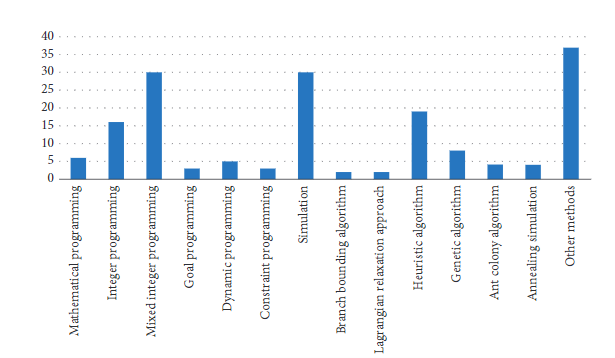
\includegraphics{graficoAlgoritmos}
    \caption{Técnicas de Optimización. Fuente \cite{Gur2018ApplicationOverview}}
    \label{GraficoTecnicasOpt}
\end{figure}

\subsection{Aproximación a la Modelización}

En función del foco a optimizar, encontramos en la literatura gran cantidad de aproximaciones a su modelización.

Podemos considerarlo como un problema de Job Shop Múltiple, o incluso como una evolución del problema de la mochila y procesamiento paralelo \cite{Lin2020AScheduling}, aunque en todos, la finalidad será la misma: \textbf{asignar un bloque de tiempo, en una sala determinada, a un paciente dado} para la realización de una intervención quirúrgica.

Dependerá, por tanto, de las restricciones y los objetivos que marquemos durante la resolución, así como de la estrategia a implementar.

\subsection{Consideraciones Finales}

Como podemos comprobar, una planificación óptima de los quirófanos constituye un rol de gran importancia en los hospitales, debido a la enorme cantidad de recursos que consumen. 

A su vez, existen gran cantidad de variables a tener en cuenta, lo cual complica \cite{Lin2020AScheduling} la optimización, pudiendo llegar a incluir tantas variables (\textit{disponibilidad de cirujanos, equipamiento, anestesistas, camas hospitalarias...}) como se desee.

En nuestro caso, nos centraremos en \textbf{asignar pacientes a huecos de quirófano}, asumiendo la disponibilidad del resto de factores, debido a que la literatura se centra en la resolución de este problema y a su dificultad de implementación.

Una vez formulado el problema con nuestras restricciones, probaremos diferentes modelizaciones y algoritmos de planificación durante el transcurso del proyecto, eligiendo finalmente el que nos ofrezca mejor rendimiento de cara a la implementación final de la herramienta.
\capitulo{7}{Conclusiones y Líneas de trabajo futuras}

Todo proyecto debe incluir las conclusiones que se derivan de su desarrollo. Éstas pueden ser de diferente índole, dependiendo de la tipología del proyecto, pero normalmente van a estar presentes un conjunto de conclusiones relacionadas con los resultados del proyecto y un conjunto de conclusiones técnicas. 
Además, resulta muy útil realizar un informe crítico indicando cómo se puede mejorar el proyecto, o cómo se puede continuar trabajando en la línea del proyecto realizado. 



\bibliographystyle{plain}
\bibliography{bibliografia}

\end{document}
